\documentclass[11pt,letterpaper]{article}

\usepackage[T1]{fontenc}
\usepackage[utf8]{inputenc}
\usepackage{lmodern}
\usepackage[margin=1in]{geometry}
\usepackage{amsmath,amssymb}
\usepackage{booktabs}
\usepackage{graphicx}
\usepackage{caption}
\usepackage[round]{natbib}
\usepackage{microtype}
\usepackage[shortcuts]{extdash}
\usepackage[hidelinks]{hyperref}
\usepackage{siunitx}
\sisetup{detect-all, group-minimum-digits=4}

\captionsetup{font=small, labelfont=bf}
\bibliographystyle{apalike}

\title{\bfseries Adjustments that do not adjust:\\
measuring shooting-foul drawing in the NBA\\
from public play-by-play}

\author{}

\date{}

\usepackage{fancyhdr}
\pagestyle{fancy}\fancyhf{}
\fancyhead[L]{\small Adjustments that do not adjust}
\fancyfoot[C]{\thepage}
\renewcommand{\headrulewidth}{0pt}

\begin{document}
\maketitle

\begin{abstract}
\noindent
How often a player draws shooting fouls, per possession he finishes, is a
strikingly stable statistic: split-half $r = 0.841$ over \num{1691} qualified
player-seasons, Spearman-Brown full-season $r = 0.914$, year-over-year
$r = 0.85$, and a padding constant of 67 possessions. We establish this on
\num{1420917} possessions from six NBA regular seasons, built entirely from
public play-by-play with no optical tracking. The natural next step is to adjust it, because a raw foul-drawing rate plainly
confounds craft with role and body type. We report that three separate
adjustments all fail, each for a reason that is visible in advance and none of
which is specific to basketball. A context model conditioning on period, clock,
score margin, venue, opponent foul rate and officiating crew reproduces the
unadjusted rate at $r = 0.995$, because an 82-game schedule averages context
away: the fitted expectation carries \SI{0.9}{\percent} of between-player
variance. Adding height and position does remove a large body-type gradient
(the correlation between the metric and height falls from $0.391$ to $0.016$),
but the result reproduces an ordinary two-variable regression residual at
$r = 0.988$. Supplying prior-season foul-drawing rate explains the signal away
by construction. We give the diagnostic that would have caught all three before
publication, and report a leakage audit of a companion model, including a
controlled retrain that moved holdout AUC from 0.6705 to 0.6578 and changed a
published leaderboard.

\end{abstract}

\noindent\textbf{Keywords:} basketball analytics; measurement reliability;
residual metrics; Poisson regression; data leakage; sports officiating

\section{Introduction}

Ask who draws the most fouls in the NBA and the raw answer is whoever shoots
most often near the basket. Free-throw attempts scale with usage and with shot
location, so the count describes a role before it describes a skill. Dividing by
possessions removes the volume part. What remains still mixes craft with
everything else that makes contact likely, and the obvious response is to model
those things and take the residual. That is the standard move in sports
analytics, from expected goals in soccer \citep{rathke2017examination,
decroos2019actions} to expected possession value in basketball
\citep{cervone2016multiresolution}.

We built that residual, and it does not work. This paper reports why, because
the reason is more useful than the metric would have been.

Two things are worth stating at the outset.

The first is a positive result and it is the foundation for everything else.
Shooting fouls drawn per finisher-possession is highly reliable at season grain.
Splitting each qualified player-season into odd and even games gives
$r = 0.841$; corrected to a full season that is $r = 0.914$; year over year it
is $0.85$. The implied padding constant is 67 possessions, so the statistic is
usable well before a season ends. None of this requires a model.

The second is the negative result, and it has three instances. We adjusted the
rate three ways and each adjustment turned out to reproduce something simpler
than itself. Conditioning on game context left the ordering essentially
untouched, at $r = 0.995$ against the unadjusted rate, because the features that
carry signal at possession grain are exactly the ones a full schedule averages
out across players. Conditioning on height and position genuinely removed a
large body-type gradient, but produced a leaderboard indistinguishable from an
ordinary weighted regression of the raw rate on height and position
($r = 0.988$, bootstrap CI $[0.985, 0.990]$). Conditioning on the player's own
prior-season rate explained the signal away, which is circular rather than
informative.

We think the general lesson transfers. A residual metric is worth building only
if the expectation it subtracts has enough between-subject variance to reorder
anybody, and that is a one-line check that almost nobody reports. Ours is
\SI{0.9}{\percent}. We give the diagnostic in Section~\ref{sec:diagnostic} and
recommend it as a precondition rather than a robustness check.

Alongside this we report a leakage audit of the companion expected field-goal
model. The public feed stamps score margin \emph{after} the event it describes,
so a feature built on it encoded the shot's own outcome. A controlled retrain on
an identical split moved holdout AUC from 0.6705 to 0.6578 and changed which
player topped a published leaderboard, while leaving calibration untouched. That
last detail is the diagnostic signature, and it is why a calibration check alone
would have missed it.

\section{Related work}

Shot quality in basketball is well covered publicly, from box-score
decomposition \citep{kubatko2007starting} to spatial models of attempt intensity
\citep{miller2014factorized} to tracking-era possession value
\citep{cervone2016multiresolution} and defensive skill recovered from defender
positions \citep{franks2015characterizing}. Shooting fouls appear inside that
tracking literature as one terminal action among several
\citep{sicilia2019deephoops}. All of that work uses inputs we do not have: the
NBA publishes tracking-derived quantities only as per-player season aggregates,
so defender distance, shot clock and touch time are unavailable per shot from
public sources.

The measurement question this paper actually turns on is treated directly by
\citet{franks2016meta}, who set out discrimination, stability and independence as
the properties a sports metric should be assessed on. Our results are best read
in that frame: the raw rate is stable and the adjusted versions are stable in
exactly the same way, which is precisely the situation their independence
criterion is designed to expose. \citet{baumer2015openwar} set the standard for
what a public, reproducible player metric looks like, and we have tried to meet
it.

Shot selection is the confound closest to our metric. \citet{sandholtz2020markov}
treat shooting decisions as a dynamic decision process and
\citet{sandholtz2020measuring} separate where a player shoots from how well he
converts. Our model conditions on context rather than on the finisher, so any
skill in \emph{choosing} contact-prone situations stays in the residual. We
return to this in Section~\ref{sec:limitations}, where it is a boundary on
interpretation rather than a defect.

On officiating, \citet{price2010racial} show NBA foul calls vary with referee and
player characteristics and \citet{pope2018awareness} show the effect attenuates
once measured publicly; \citet{anderson2009officiating} and
\citet{price2012subperfect} document that calls respond to game state and score
differential. \citet{dohmen2016referee} survey the field. We use crew foul rate
as a feature for this reason and report in Section~\ref{sec:officiating} why the
resulting coefficient supports much less than it appears to.

Two methodological strands complete the picture. Calibration of probabilistic
predictions is long-established \citep{brier1950verification} and the correction
we apply is standard \citep{zadrozny2002transforming}, with boosted models
particularly needing it \citep{niculescu2005predicting, guo2017calibration}.
Leakage has a formal taxonomy \citep{kaufman2012leakage} and a documented role in
irreproducible machine-learning results \citep{kapoor2023leakage};
Section~\ref{sec:audit} is an instance found in a public sports feed.

\paragraph{What we could not find, and a caveat about how we looked.}
We found no public, reproducible model of expected free-throw attempts that
reports the reliability of the resulting player metric. That claim is weaker than
it may appear. Our bibliography was assembled programmatically against CrossRef
and OpenAlex, which index machine-learning methodology, soccer analytics and
referee economics well and applied basketball analytics poorly, because much of
that work lives in conference proceedings, books and public websites that
neither service covers. Readers should treat the gap as unverified rather than
established. In particular, free-throw rate as a normalisation is standard
practice descending from the Four Factors, several public all-in-one player
metrics publish projected free-throw rates, and at least one public analytics
site publishes filtered foul-drawn rates with positional percentiles. We do not
claim priority over any of it.

\section{Data}

\subsection{Sources and construction}

Everything is built from two public NBA Stats endpoints: the V3 live
play-by-play feed and \texttt{shotchartdetail}, which supplies shot coordinates
and zone labels. No optical tracking is used. Possessions are split with the
\texttt{pbpstats} library rather than by custom logic, so the possession
definition is one other researchers can reproduce.

The corpus covers six regular seasons, 2020--21 through 2025--26: \num{7230}
games (\num{1080} in the COVID-shortened 2020--21 and \num{1230} in each
subsequent season), \num{1420917} possessions and \num{1282312} field-goal
attempts.

\subsection{Target definition}

The modelled quantity, \texttt{sfta}, counts free-throw attempts awarded on a
shooting foul, including the single bonus shot of an and-one. Technical,
flagrant, clear-path, away-from-play, inbound and penalty (non-shooting-foul
bonus) free throws are excluded, because they are not caused by the act of
shooting. Of the free throws in the corpus, \num{255738} are kept and \num{67569}
excluded. A further 533 trips were dropped as contaminated, mostly misclassified
and-ones, an audit rate of \SI{0.085}{\percent}.

The distribution is lumpy. Across \num{1420917} possessions the target takes
value 0 on \num{1278429}, 1 on \num{34460}, 2 on \num{103037}, 3 on \num{4769},
4 on 213 and 5 on 9. Two is roughly three times more common than one, because a
shooting foul on a missed two-point attempt awards two shots while an and-one
awards one. The identity
$\texttt{sfta} = \texttt{ft\_and1} + \texttt{ft\_sf2} + \texttt{ft\_sf3}$ holds
on every row.

\paragraph{Scope.} This is shooting-foul drawing, not foul drawing. Penalty free
throws are \SI{21}{\percent} of drawn free throws and drawing a reach-in on a
drive in the bonus is foul-drawing skill by any ordinary definition. The
exclusion is right for the causal question (only shooting fouls are caused by the
shot) but it is a real narrowing, and it is not random across players: whether
contact is scored as a shooting foul or a common foul in the penalty is partly an
officiating judgement, and a player whose team reaches the bonus early has more
of his drawn contact converted into excluded attempts. We have not run the
all-fouls sensitivity check this warrants.

\subsection{Attribution}

A possession is attributed to a finisher: the free-throw shooter when a
qualifying trip occurred, otherwise the last player to make a shot, otherwise the
player who turned the ball over, otherwise the last shooter. Every fouled
possession has a finisher; \SI{98.0}{\percent} of all possessions do, leaving
\num{1392350} attributable possessions, of which \num{1384016} join to a
player-season record.

Note that the numerator partly determines the denominator: drawing a shooting
foul creates an attributed possession. The denominator is close to a standard
usage denominator, and we have not checked robustness against one that does not
depend on the outcome.

Players qualify at 300 finisher-possessions, giving \num{1691} qualified
player-seasons drawn from 546 distinct players. That clustering matters for
uncertainty and we handle it in Section~\ref{sec:reliability}.

\section{The statistic, and the models fitted to adjust it}

The unadjusted quantity is shooting-foul free throws per 100 finisher
possessions. Across qualified player-seasons its mean is 17.89 and its standard
deviation 7.58.

Each adjusted version subtracts a fitted expectation and is reported per 100
possessions. All models share a six-fold season cross-fit (train on five seasons,
predict the sixth) and per-season scaling of predictions to the observed league
rate. Three specifications:

\begin{description}
\item[Context] a Poisson generalised linear model \citep{nelder1972generalized}
at possession grain on period, seconds remaining, score margin at possession
start, a fourth-quarter/overtime indicator, whether the offence is at home, the
defending team's season shooting-foul rate, and the mean season rate of the three
assigned officials. The two rate features are leave-one-game-out.
\item[Body type] the same, plus the finisher's height and position.
\item[Identity] the same again, plus the finisher's prior-season free-throw
rate, mean-imputed from training seasons with a missingness indicator.
\end{description}

We also fit two alternative learners on the context specification: a multinomial
logit over $\{0,1,2,3^{+}\}$ with the top class valued at its training-fold mean,
and a Poisson LightGBM \citep{ke2017lightgbm} early-stopped on a random
\SI{10}{\percent} of training rows.

\paragraph{A correction to the fitting universe.}
Our original specification fitted on all \num{1420917} possessions, including
\num{28567} with no finisher that carry \texttt{sfta} $= 0$ by construction.
Those structural zeros bias the fitted mean down by exactly the universe ratio
$\num{1420917}/\num{1392350} = 1.0205$, and the per-season scaling factors were
correspondingly $1.013$ to $1.025$, mean $1.0204$. We had attributed those
factors to league-wide enforcement drift. They were an artifact. Refitting on
attributable possessions moves the factors to a mean of $0.9987$, and no season
shows the signature of the 2021--22 crackdown on non-basketball shooting motions
under either specification. We report this because the erroneous interpretation
survived our own pre-publication audit and was caught only in review.

\section{The statistic is reliable}
\label{sec:reliability}

Splitting each qualified player-season into odd and even games and correlating
across halves gives $r = 0.841$ for the unadjusted rate. The Spearman-Brown
full-season figure is $r = 0.914$ \citep{spearman1910correlation, brown1910some},
the implied padding constant is $K = 67$ possessions, and year-over-year
correlation averages $0.85$ across five consecutive-season pairs (0.852, 0.834,
0.859, 0.865, 0.840).

Three qualifications, none of which we found in our own first draft.

\emph{Uncertainty.} The \num{1691} player-seasons come from 546 players, so they
are not independent. A player-clustered bootstrap (2{,}000 replicates) gives
$r = 0.841$ with 95\% CI $[0.815, 0.863]$ and full-season $0.914$
$[0.898, 0.926]$. The naive interval is too narrow. $K = 67$ has CI $[57, 80]$.

\emph{Split design.} Alternating games balances within-season nonstationarity away.
A chronologically blocked split (first half of the season against second) gives
$r = 0.808$ and $K = 84$. That is the more honest test-retest and it is still
high. A method-of-moments calculation predicts $r = 0.835$ from pure sampling
error alone, so the excess over sampling noise is $+0.006$: there is no material
inflation from shared opponents, shared crews or the shared scaling constant.

\emph{Practical reading.} A player reaches $r = 0.9$ at roughly 600 possessions
under the alternating split, but the defensible range across estimator choices is
about 500 to 760. Qualified players average 709 finisher-possessions across 63
games, so 600 possessions is about 53 games, not the two months an earlier draft
of this paper claimed. Two months of a rotation player's usage gives $r$ near
$0.82$.

\begin{figure}[t]
\centering
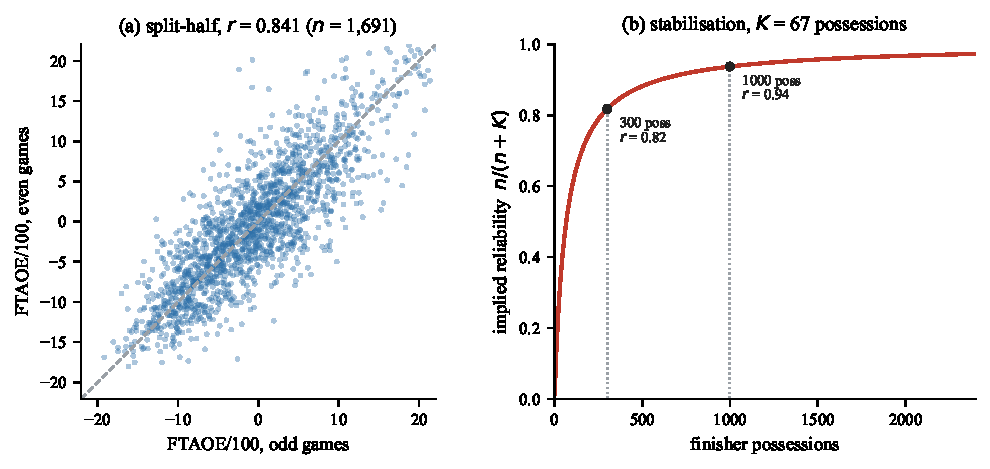
\includegraphics[width=\textwidth]{figures/fig2_ftaoe_reliability.pdf}
\caption{Season-level reliability. (a) Odd-game against even-game rate for
\num{1691} qualified player-seasons. (b) Implied reliability against sample size,
$n/(n+K)$ with $K = 67$.}
\label{fig:rel}
\end{figure}

\section{Three adjustments, and what each one reproduces}
\label{sec:adjustments}

\subsection{Context reproduces the unadjusted rate}

The context model improves on a season-mean baseline by \SI{0.195}{\percent} of
the reported criterion. Clustered by game, that is distinguishable from zero
(95\% CI \SI{0.180}{\percent} to \SI{0.212}{\percent}, $t = 23.9$); the problem
is effect size, not significance.

The problem is visible in one comparison. Across player-seasons the fitted
expectation has a standard deviation of \textbf{0.73} per 100 against an observed
standard deviation of \textbf{7.58}. It carries \SI{0.9}{\percent} of the
between-player variance. Subtracting it therefore cannot reorder anyone:
correlation with the unadjusted rate is $r = 0.995$, top-20 overlap 16 of 20, and
the mean within-season rank movement is 1.7 places (Table~\ref{tab:adjust},
Figure~\ref{fig:adjust}a).

It follows that the reliability figures in Section~\ref{sec:reliability} are
properties of the unadjusted rate, not achievements of the model. Measured
directly, the unadjusted rate returns split-half $0.8410$, full-season $0.9136$
and year-over-year $0.8491$, against $0.8408$, $0.9135$ and $0.8497$ for the
adjusted version. The raw rate is marginally the more reliable of the two.

The reason is structural and worth stating, because it is the transferable part.
The only two features carrying meaningful weight are the opponent's and the
crew's season foul rates. Over 82 games every player faces close to the same
distribution of both, so features that are genuinely informative about an
individual possession have almost no variance across players once a season is
aggregated. The model is not broken; it is answering a question whose answer is
nearly constant at the grain the metric is used.

\subsection{Body type reproduces a two-variable regression}

The unadjusted rate has a large, monotone height gradient: $r = 0.391$ with
finisher height ($r^2 = 0.153$). Mean rate by height band runs from $-4.31$ per
100 for players 6\,ft\,2\,in and under to $+5.76$ for players 7\,ft and over, a
spread of $10.07$ on a statistic whose standard deviation is $7.57$
(Figure~\ref{fig:height}). Roughly \SI{15}{\percent} of the variance is body
type, which no definition of foul-drawing craft includes.

Adding height and position removes it: the correlation with height falls to
$0.016$. That is a real improvement and it is the specification we expected to
ship.

It does not survive the obvious comparison. Regressing the unadjusted rate on
height and position within season, weighted by possessions, and taking the
residual is a calculation requiring no model, no possession grain and no context
features at all. The body-type specification reproduces that residual at
$r = 0.988$, player-clustered bootstrap CI $[0.985, 0.990]$, with 18 of 20
top-20 members shared. Both move the metric away from the unadjusted rate by
almost exactly the same amount ($r = 0.917$ and $0.914$ respectively).

\subsection{Identity explains the signal away}

Adding the finisher's prior-season free-throw rate raises fit further and drops
rank correlation with the context specification to $\rho = 0.832$. This is
circularity rather than improvement: prior-season rate is a measurement of the
thing being measured. Rudy Gobert's 2022--23 season moves from $+20.06$ to
$-15.70$ per 100, the largest change in the sample, and he supplies four of the
eight largest drops. Told in advance that Gobert draws fouls at a high rate, the
model expects it, and he stops exceeding expectation.

We note the tension with Section~\ref{sec:reliability}, because an earlier draft
of this paper did not. Year-over-year persistence of $0.85$ is cited there as
evidence the statistic measures something real, and here the predictive power of
prior-season information is rejected as circular. Both readings cannot be
load-bearing. The consistent position is the narrow one: persistence establishes
that the quantity is stable, and stability is equally consistent with measuring a
durable role or body type, which Section~\ref{sec:adjustments} shows is
substantially what it does measure.

\begin{table}[t]
\centering
\small
\caption{What each adjustment reproduces. All at qualified player-season grain
($\geq 300$ possessions, $n = \num{1691}$ from 546 players). Intervals are
player-clustered bootstrap, 2{,}000 replicates.}
\label{tab:adjust}
\begin{tabular}{llccc}
\toprule
Adjustment & Compared against & Pearson $r$ & 95\% CI & Top-20 \\
\midrule
Context & unadjusted rate & \textbf{0.995} & $[0.995, 0.996]$ & 16/20 \\
Body type & linear height + position residual & \textbf{0.988} & $[0.985, 0.990]$ & 18/20 \\
Body type & unadjusted rate & 0.917 & $[0.901, 0.931]$ & 10/20 \\
Linear residual & unadjusted rate & 0.914 & $[0.899, 0.928]$ & 12/20 \\
Identity & context adjustment & 0.810 & --- & --- \\
\bottomrule
\end{tabular}
\end{table}

\begin{figure}[t]
\centering
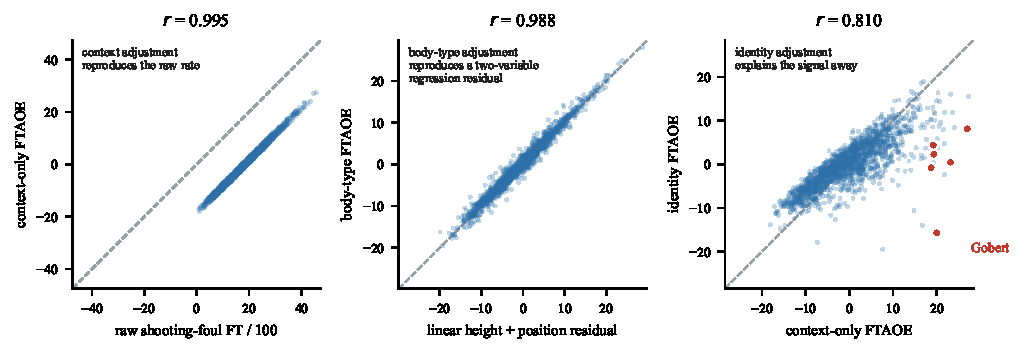
\includegraphics[width=\textwidth]{figures/fig3_adjustments.pdf}
\caption{Each adjustment against what it reproduces. (a) The context model
against the unadjusted rate. (b) The body-type model against an ordinary
weighted regression residual on height and position. (c) The identity model
against the context model, with Gobert's six seasons marked.}
\label{fig:adjust}
\end{figure}

\begin{figure}[t]
\centering
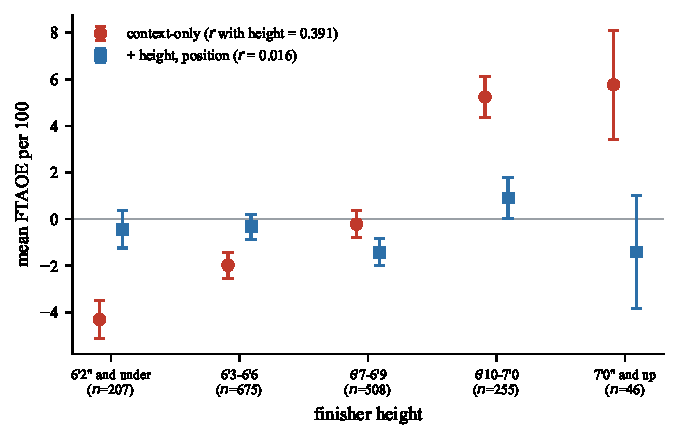
\includegraphics[width=0.62\textwidth]{figures/fig4_height_gradient.pdf}
\caption{Mean adjusted rate by finisher height, with 95\% intervals. The context
specification carries the full body-type gradient; adding height and position
removes it, and reproduces a two-variable regression in doing so.}
\label{fig:height}
\end{figure}

\subsection{Two alternative learners change nothing}

The multinomial specification produces a rank-identical leaderboard
($\rho = 1.0000$, 20 of 20). This is close to tautological rather than
informative: an essentially unpenalised multinomial logit whose expectation is a
probability-weighted class value over the same seven-feature linear index
recovers the same conditional mean, so it does not test the lumpy-support
question it was introduced to test.

The Poisson LightGBM improves the criterion to \SI{0.254}{\percent} and produces
a leaderboard at $\rho = 0.9988$. Its per-fold values are 0.294, 0.253, 0.246,
0.323, 0.323 and 0.097, and we report the last one because reporting only the
mean would hide it. An earlier draft justified keeping the GLM on the grounds
that the boosted model calibrated worse; Section~\ref{sec:calibration} withdraws
that justification. The GLM is retained for parsimony, and because at
$\rho = 0.9988$ the choice is immaterial.

\section{A diagnostic that would have caught all three}
\label{sec:diagnostic}

Every failure above is detectable before any modelling, from two numbers:

\begin{enumerate}
\item $\operatorname{Var}(\hat{\mu}) / \operatorname{Var}(y)$ at the grain the
metric is consumed, where $\hat\mu$ is the fitted expectation. Ours is
\num{0.0093}. An expectation carrying under a few per cent of between-subject
variance cannot reorder subjects, whatever its fit statistic says.
\item The correlation between the proposed residual and the simplest thing it
could have been: the unadjusted rate, and any trivial regression on the
covariates the model adds. Ours are $0.995$ and $0.988$.
\end{enumerate}

Neither requires new data and both are one line. We recommend reporting them as a
precondition for a residual metric rather than as a robustness check, and we note
that per-event fit statistics such as deviance lift give no warning at all: our
criterion was significantly non-zero throughout.

\section{The leakage audit}
\label{sec:audit}

We audited the pipeline against a fixed checklist before publication: target
definitions, per-row identities, duplicate keys, prediction coverage, feature
timing, split construction, comparison against published league aggregates,
direction checks, and missing-data handling. The audit found four substantive
problems and missed two more that review caught, which we report in that order.

\paragraph{The score-margin leak (critical).} The \texttt{score\_margin} field on
a shot row is stamped after the event resolves, so for a made shot it already
contains that shot's points. Our expected field-goal model used a derived feature
built on it. We confirmed the timing against the play-by-play sequence and
retrained on an identical split. Holdout AUC fell from 0.6705 to 0.6578.
Calibration was essentially unaffected, expected calibration error moving from
0.0040 to 0.0042, and that is the diagnostic signature: the leak inflated ranking
without distorting the probability scale, so a calibration check alone would have
missed it. The 2024--25 leader in points over expected per 100 changed from Jimmy
Butler III (23.82) to Ty Jerome (22.99), with Butler at 22.42 corrected. We report
the flip because it happened, not as evidence of magnitude: the gap between first
and second is 0.57 and we have not established that the metric resolves
differences that small.

\paragraph{Missing season scaling on xFG (meaningful).} League-wide field-goal
points over expected per 100 ranged from $-1.70$ to $+1.07$ across seasons when it
should sit near zero; per-season scaling reduced the range to $-0.25$ to $+0.42$.

\paragraph{A flat free-throw baseline (meaningful).} Drawn free throws were valued
at a hardcoded \SI{77}{\percent} against actual league rates of
\SI{77.5}{\percent} to \SI{78.4}{\percent}.

\paragraph{A second margin leak, immaterial in effect (real).} The possession
margin used by the foul model was stamped on the terminal event and was null on
non-scoring possessions, so the filled value half-encoded whether the possession
scored. Refitting on the possession-start margin changed no player-season by more
than 1.03 free throws, moved no player into or out of any season's top 20, and
shifted no rank by more than five places. Two leaks of the same class had very
different consequences and only measurement distinguished them.

\paragraph{What the audit missed.} Two things, both found in review. The fitting
universe error described in Section~4 produced scaling factors we misread as
league drift. And the leave-one-game-out rate features are computed within each
season including the held-out one, so while the coefficients are out-of-fold the
features are not. An ablation quantifies the cost: the four base features alone
give \SI{0.153}{\percent}, the shipped specification \SI{0.196}{\percent}, and
rebuilding the rate features from training seasons only gives
\SI{0.146}{\percent}. The rate features contribute roughly a fifth of the reported
figure, and that contribution is entirely same-season target information. The
\SI{0.195}{\percent} is therefore retrospective, not prospective. In a paper whose
methods contribution is feature timing, this is the place we applied a looser
standard to ourselves than to the feed.

We also note that the criterion we report as ``Poisson deviance'' omits the
saturated-model term and is therefore $2\times$ the negative log-likelihood. The
deviance \emph{drop} is unaffected; on the true deviance the lift is
\SI{0.227}{\percent} rather than \SI{0.195}{\percent}. The error runs in the
conservative direction. We report both and use the conservative figure throughout.

\section{Calibration}
\label{sec:calibration}

Aggregate calibration holds and is partly guaranteed by the per-season scaling:
over player-seasons with at least 100 possessions, mean predicted rate is 0.1835
against 0.1853 observed, a gap of \SI{0.95}{\percent}.

Calibration across predicted deciles depends on the estimator, and an earlier
draft of this paper reported the wrong one as a finding. At the qualifying
threshold the metric is actually used at, with a possession-weighted regression,
the slope is $1.011$ (95\% CI $[0.512, 1.509]$). An unweighted regression over ten
decile means, computed on a sample that also includes 797 sub-threshold
player-seasons, gives $0.426$ with CI $[-0.288, 1.139]$ and $p = 0.206$. The
second is not a finding; it is a noisier estimator on a wider sample, and its own
interval contains one. We had reported it as evidence of weak calibration and
defended it with an appeal to regression dilution, which is also wrong: dilution
requires measurement error in the predictor, and a narrow predictor range inflates
a slope's standard error without biasing it.

\section{Officiating}
\label{sec:officiating}

The crew rate coefficient is real. Clustered by game it runs $z = 5.0$ to $7.2$
across folds. It supports considerably less than that suggests.

Official-level foul rates are themselves unstable: within-season odd/even
split-half $r = 0.508$, and year-over-year $r = 0.178$ across the five pairs
(0.254, 0.185, 0.150, 0.139, 0.162). For comparison the defensive-team rate
splits at $0.688$. An official's shooting-foul tendency is roughly half noise
within a season and essentially does not persist between them. That is consistent
with the ablation result above, where an honestly out-of-fold crew feature adds
nothing.

Three consequences. The within-season crew term is a description of the games a
crew happened to work, not a forecastable tendency. It cannot be used to
apportion a player's season variance between officiating and his own play, and an
earlier draft proposed exactly that. And no claim about bias is available here:
crew assignment is not random with respect to teams, venues or scheduling.

The score-margin coefficient deserves a plainer statement than we first gave it.
Cluster-robust standard errors put every fold's estimate within one standard error
of zero ($z$ from $0.07$ to $0.88$). We described this as instability across
folds. It is a null, and it should be reported as one.

\section{Limitations}
\label{sec:limitations}

\paragraph{The metric is not craft.} Section~\ref{sec:adjustments} shows the
unadjusted rate is substantially body type and role, and that neither adjustment
we tried isolates anything else. We make no claim that any quantity in this paper
measures foul-drawing skill net of the things that make contact likely.

\paragraph{Shot selection sits in the residual.} Because the models condition on
context rather than on the finisher, skill in choosing contact-prone situations is
never subtracted. Separating it needs a shot-selection model
\citep{sandholtz2020measuring} we have not built, and there is a real obstacle:
conditioning on the observed shot selects on the outcome, since a shooting foul
frequently corrupts or replaces the recorded field-goal attempt. We flag that as
the reason a location-conditioned specification is not simply a matter of adding
features.

\paragraph{No tracking data.} Defender distance, contest, shot clock and touch
time are unavailable per shot publicly. This caps the companion shot model near
AUC 0.66 \citep{cervone2016multiresolution} and removes the most plausible
physical mediator of foul drawing.

\paragraph{Bonus state is unobserved.} The public feed carries no bonus indicator,
so a fourth\-/quarter or overtime flag stands in for it.

\paragraph{Single-season xFG benchmark.} The leakage comparison rests on one
holdout season, 2024--25. The reliability results use all six seasons.

\paragraph{Specification search.} Four feature sets and five variant arms were
evaluated on the same six seasons. With effects this small, selecting among them
on the same data is not a negligible bias. We have not reserved an untouched
holdout season, and future work on this pipeline should.

\paragraph{Coverage gaps.} About \num{1800} shots per season in 2021--22 through
2024--25 (\SI{0.8}{\percent}) carry no location and are excluded from xFG. A
2025--26 change in how end-of-period heaves are charged creates a cross-season
discontinuity in long-range attempts.

\section{What this leaves a practitioner}

The usable output is the unadjusted statistic with a known error curve. Shooting
fouls drawn per 100 finisher possessions is reliable at $r = 0.914$ over a
season, persists year to year at $0.85$, and stabilises with a padding constant of
67 possessions, so a shrunk estimate is meaningful by roughly a third of a season.
Use it shrunk, per 100, and with the understanding that a substantial part of what
it measures is how tall a player is and where he plays.

What we cannot offer is the adjusted version. Anyone wanting foul-drawing net of
body type should run the two-variable regression, which performs
indistinguishably from our model and takes a minute. Anyone wanting foul-drawing
net of shot selection is looking at an unsolved problem with a real
selection-on-outcome obstacle in the way.

The transferable contribution is Section~\ref{sec:diagnostic}. Before building a
residual metric, check whether the expectation has enough between-subject variance
to reorder anybody, and check the residual against the simplest thing it could
have been. Both are one line, and either would have saved this project a model.

\section*{Reproducibility}

All model artifacts, validation scripts and the code producing every figure and
table are in a public repository, withheld here for anonymous review and
supplied to the editor. The variant comparisons each
assert that their baseline arm reproduces the shipped model before their variant
arms are read. The bibliography was generated programmatically from records
resolved against CrossRef and OpenAlex, with the coverage caveat noted in
Section~2. Package versions are not currently pinned and the derived
possession-level table is not archived; both should be fixed before this work is
relied upon, and the \texttt{pbpstats} version in particular is load-bearing
because the possession definition underlies every number here.

\bibliography{references}

\end{document}
